\documentclass[10pt]{article}
\usepackage{amsmath}
\usepackage{amsfonts}
\usepackage{amssymb}
\usepackage{amsthm}
\usepackage{graphicx}   %Include graphics
\usepackage{float}      %Used to force graphics to stay where I want them to stay
\usepackage{mathrsfs}   %for Fourier transform 'F' symbol \mathscr{F}
\usepackage{hyperref}   %For hyperlinks in the PDF
\usepackage{enumitem}   %so we can have nonIndented lists and enumerations
\usepackage{caption}
\usepackage{subcaption}


\pdfpagewidth 8.5in
\pdfpageheight 11in
\setlength{\oddsidemargin}{-.35in}
\setlength{\textwidth}{7.32in}
\setlength{\topmargin}{-.6in}
\setlength{\textheight}{9.4in}

%%%%%%%%%%%%%%%%%%%%%%%%%%%%%%%%%%%%%%%%%%%%%%%%%%%%%%%%%%

%matrix macro
\newcommand{\mat}[2][ccccccccccccccc]{\left [\!\!\begin{array}{#1} #2\\ \end{array} \!\!\right]}
\newcommand{\determ}[2][ccccccccccccccc]{\left| \begin{array}{#1} #2\\ \end{array} \right| \vspace{.5em}}

%permutation
\newcommand{\perm}[2][ccccccccccccccc]{\left (\begin{array}{#1} #2\\ \end{array} \right) \vspace{.5em}}

%piecewise function
%  example:
%     $$H_i(K, K_0)\iso\piece{ \trivial & \text{if $i=0$} \\ \bbz/2\bbz &\text{if $i=1$} \\ \trivial & \text{if $i\ge2$}}$
%
\newcommand{\piece}[2][cll]{\left \{\begin{array}{#1} #2\\ \end{array} \right. }

%system of equations
\newcommand{\sys}[2][lll]{\left \{\begin{array}{#1}#2 \\ \end{array} \right. }

%integral
\newcommand{\dint}{\displaystyle\int}

%sum
\newcommand{\dsum}[3]{
           \displaystyle\sum_{#1}^{#2} #3 }

%sum start i=0
\newcommand{\dsumiz}[2]{
           \displaystyle\sum_{i=0}^{#1} #2}

%sum start i=1
\newcommand{\dsumio}[3]{
           \displaystyle\sum_{i=1}^{#2} #3 }


%sets {b,...,e} and sets with conditions {x | x is an integer}
\newcommand{\set}[2]{  \left\{#1,\ldots,#2\right\} }
\newcommand{\dset}[2]{  \left\{#1\; :\;\;#2\right\} }
\newcommand{\plist}[2]{  \left(#1,\ldots,#2\right) }

\newcommand{\iso}{\cong}
\newcommand{\abs}[1]{ \left|#1\right|}
\newcommand{\pdfrac}[2]{\!\left(\dfrac{#1}{#2}\right)\! }
\newcommand{\pfrac}[2]{\!\left(\frac{#1}{#2}\right)\! }

\newcommand{\libzptrl}[2]{\dfrac{\partial #1}{\partial #2} }
\newcommand{\plibzptrl}[2]{\left(\dfrac{\partial #1}{\partial #2}\right) }
\newcommand{\libz}[2]{\dfrac{d #1}{d #2} }
\newcommand{\plibz}[2]{\left(\dfrac{d #1}{d #2}\right) }
\newcommand{\eval}[2]{\bigg|_{#1}^{#2}}
\newcommand{\transpose}[1]{{#1}\!^T\!}

\newcommand{\mean}{\mbox{E}}
\newcommand{\var}{\mbox{V}}
\newcommand{\cor}{\mbox{Cor}}

\newcommand{\inn}{^{\mbox{inn}}}
\newcommand{\out}{^{\mbox{out}}}
\newcommand{\innL}{^{\mbox{innL}}}
\newcommand{\innR}{^{\mbox{innR}}}
\newcommand{\outL}{^{\mbox{outL}}}
\newcommand{\outR}{^{\mbox{outR}}}
\newcommand{\iloe}{^{\mbox{iloe}}}
\newcommand{\olie}{^{\mbox{olie}}}
\newcommand{\iloeL}{^{\mbox{iloeL}}}
\newcommand{\iloeR}{^{\mbox{iloeR}}}
\newcommand{\olieL}{^{\mbox{olieL}}}
\newcommand{\olieR}{^{\mbox{olieR}}}
\newcommand{\m}{^{{\mbox{m}}}}
\newcommand{\mL}{^{{\mbox{mL}}}}
\newcommand{\mR}{^{{\mbox{mR}}}}
\newcommand{\comp}{^{{\mbox{c}}}}
\newcommand{\inv}{^{-1}}
\newcommand{\pprime}{^{\prime\prime}}
\newcommand{\erf}{\mbox{Erf}\,}
\newcommand{\Span}{\mbox{span}}

\newcommand{\trivial}{\{0\}}						%trivial group (abelian) {0}
\newcommand{\cbrace}[1]{\left\{#1\right\}}				%curly-braces {parameter}
\newcommand{\gen}[1]{\left\langle#1\right\rangle}
\newcommand{\norm}[1]{\left|\left|#1\right|\right|}
\newcommand{\dsup}[1]{displaystyle{\sup_{#1}}}
\newcommand{\range}{\mathrm{range}\;}
\newcommand{\trace}{\mathrm{trace}\;}
\newcommand{\lcm}{\mathrm{lcm}\;}
\newcommand{\clos}{\mathrm{clos\!}\;}
\newcommand{\supnorm}[1]{\norm{#1}_\infty}
\newcommand{\clin}{\mathrm{clin\!}\;}
\newcommand{\lin}{\mathrm{lin\!}\;}

\newcommand{\tuple }[2]{\left(#1, #2\right)}
\newcommand{\paren}[1]{\!\left(#1\right)\!}
\newcommand{\bracket}[1]{\left[#1\right]}
\newcommand{\inprod}[2]{\left\langle#1,#2\right\rangle}

\renewcommand\Re{\operatorname{Re}}
\renewcommand\Im{\operatorname{Im}}

\newcommand{\degree}{\ensuremath{^\circ}}
\newcommand{\overbar}[1]{\mkern 1.5mu\overline{\mkern-1.5mu#1\mkern-1.5mu}\mkern 1.5mu}
\newcommand{\Lim}[1]{\raisebox{0.5ex}{\scalebox{0.8}{$\displaystyle \lim_{#1}\;$}}}


%%%%%%%Boxes%%%%%%%%%%%%%%
\newcommand{\fpbox}[2]{
       \fbox{\parbox{#1}{#2}}
}
\newcommand{\cfbox}[1]{
\begin{center}
       \fbox{#1}
\end{center}
}
%%%%%%%%%%%%%%%%%%%%%%%%%%


%black board font
\newcommand{\bbc}{\mathbb{C}}
\newcommand{\bbd}{\mathbb{D}}
\newcommand{\bbf}{\mathbb{F}}
\newcommand{\bbn}{\mathbb{N}}
\newcommand{\bbz}{\mathbb{Z}}
\newcommand{\bbq}{\mathbb{Q}}
\newcommand{\bbr}{\mathbb{R}}
\newcommand{\bbt}{\mathbb{T}}
\newcommand{\bbx}{\mathbb{X}}
\newcommand{\bbu}{\mathbb{U}}

%script font
\newcommand{\sca}{\mathcal{A}}
\newcommand{\scb}{\mathcal{B}}
\newcommand{\scs}{\mathcal{S}}
\newcommand{\scl}{\mathcal{L}}
\newcommand{\scu}{\mathcal{U}}
\newcommand{\scm}{\mathcal{M}}
\newcommand{\sck}{\mathcal{K}}
\newcommand{\scf}{\mathcal{F}}
\newcommand{\sch}{\mathcal{H}}

\newcommand{\KL}{\mathcal{KL}}

 \renewcommand{\i}{\mathrm{i}}

\newcommand{\tinyspace}{5em }
\newcommand{\mediumspace}{10em }
\newcommand{\largespace}{10em }
\newcommand{\largerspace}{20em }
\newcommand{\hugespace}{40em }
\newcommand{\seperator}{\underline{\hspace{45em}}}

%%%%%%%%%%%%%%%%%%%%%%%%%%%%%%%%%%%%%%%%%%%%%%%%%%%%%%%%%%

%stretch rows of a table
\renewcommand*\arraystretch{1.10}

\pagestyle{plain}
\begin{document}

    \title{AMS 232 Nonlinear Optimization \#1}
    \author{Harleigh Marsh}
    \date{\today}
    \maketitle


%Problem Set
\begin{enumerate}[leftmargin=*]
  \item Consider a full-rank matrix $A\in\bbr^{m\times n}$ where $n\ge m$, let $b\in\bbr^n$ and $x\in\bbr^m$.  Using necessary conditions, solve the following problem:
      \begin{equation*}
        \begin{aligned}
            & \underset{x}{\text{minimize}}
            & & (Ax-b)^T(Ax-b)
        \end{aligned}
      \end{equation*}

      Define $f:\bbr^m\longrightarrow\bbr$ as $f(x)=(Ax-b)^T(Ax-b)$, then our problem can be written nicely as
      \begin{equation} \label{eq:p1}
        \begin{aligned}
        & \underset{x}{\text{minimize}}
        & & f(x) \\
        & \text{subject to}
        & & x\in\bbr^m
        \end{aligned}
      \end{equation}
      As \ref{eq:p1} is unconstrained, a first order necessary condition is given as if $x$ is a local minimum then $\libzptrl{f}{x}=0$.  Therefore we need but compute the gradient of $f$ and set it to zero.
      \begin{align*}
         0 &= \libzptrl{f}{x}\\
           &= \libzptrl{}{x}\paren{(Ax-b)^T(Ax-b)}\\
           &= \libzptrl{}{x}\paren{ x^TA^TAx - x^TA^Tb-b^TAx + b^Tb }\\
           &= 2x^TA^TA - b^TA - b^TA + 0\\
           &= 2x^TA^TA - 2b^TA
      \end{align*}
      Therefore, since the inverse and transpose operators commute, we have that $x=(A^TA)\inv A^Tb$, which is our necessary condition.

  \item Apply necessary conditions on the following optimization problem where $A\in\bbr^{n\times m}$ is full-rank with $n< m$, and $b\in\bbr^n$ and $x\in\bbr^m$
      \begin{equation} \label{eq:p2}
        \begin{aligned}
        & \underset{x}{\text{minimize}}
        & & x^Tx \\
        & \text{subject to}
        & & Ax=b
        \end{aligned}
      \end{equation}
      As we have an equality constraint $Ax-b=0$ we apply the necessary condition of Lagrange, which requires that at an optimal point $\libzptrl{\scl}{x}$ and $\libzptrl{\scl}{\lambda}$.  Building the Lagrangian, we have
      \begin{align*}
        \scl &= x^Tx - \lambda^T(Ax-b) \tag{where $\lambda\in\bbr^n$}\\
          &= x^Tx - \lambda^TAx + \lambda^Tb
      \end{align*}
      Therefore
      \begin{align*}
        0 &= \libzptrl{\scl}{x} = 2x^T-\lambda^TA &\rightarrow&& x=\frac{1}{2}A^T\lambda \tag{$\alpha$}\\
        0 &= \libzptrl{\scl}{\lambda} = Ax-b  &\rightarrow&& Ax=b  \tag{$\beta$}
      \end{align*}
      Now with ($\alpha$) into ($\beta$) we solve for $\lambda$ as $\lambda=2(AA^T)\inv b$, and so putting this back into ($\alpha$) we get the necessary condition
      \begin{align*}
        x = A^T(AA^T)\inv b
      \end{align*}

  \item Here we answer the following out of Nocedal and Wright's Numerical Optimization text:
                     \begin{figure}[H]
                        \centering
                        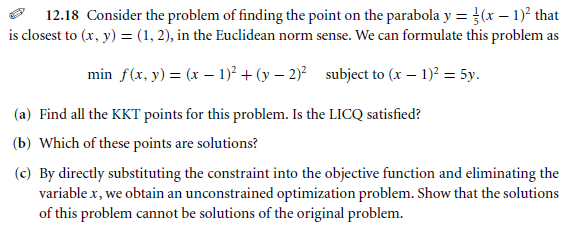
\includegraphics[width=.5\textwidth]{prob3.png}
                      \end{figure}
        With a slight change of notation of $x = \mat{x_1\\x_2}$, we have
        \begin{equation} \label{eq:p3}
        \begin{aligned}
        & \underset{x}{\text{minimize}}
        & & f(x)\triangleq(x_1 - 1)^2 + (x_2-2)^2 \\
        & \text{subject to}
        & & (x_1-1)^2-5x_2=0
        \end{aligned}
      \end{equation}


      (a):
        In \ref{eq:p3} we have only one equality constraint, we have, with $\lambda\in\bbr$  that the Lagrange function is
        $\scl(x, \lambda) = (x_1 - 1)^2 + (x_2-2)^2 - \lambda( (x_1-1)^2-5x_2)$.  Applying the KKT conditions gives
        \begin{align*}
            \libzptrl{\scl}{x}=0 \\
            (x_1-1)^2-5x_2=0
        \end{align*}
        Therefore we have three equations
        \begin{align*}
            \mat{2(x_1-1)-2\lambda(x_1-1) \\ 2(x_2-2)+5\lambda} = \mat{0\\0}\\
            (x_1-1)^2-5x_2=0
        \end{align*}
        Solving this system, we get only one real solution, $x^*=\mat{x_1^*\\x_2^*}=\mat{1\\0}$.  Lastly, we show that LICQ holds at $x^*$.  Computing the gradient of the (only) constraint at $x^*$ gives
        \begin{align*}
            \libzptrl{}{x}((x_1-1)^2-5x_2)\eval{x=x^*}{} = \mat{2(x_1-1)\\-5}_{|{x=x^*}}=\mat{0\\-5}
        \end{align*}
        which is clearly linearly independent.  Therefore LICQ holds at $x^*$.

        (b):  To show that the point we found in (a), $x^*=\mat{1\\0}$, we apply the second order sufficient conditions for KKT (given as theorem 12.6 in the text). With $x^*$ we get $\lambda^*=\frac{4}{5}$.  Now, computing the Hessian of $\scl$ and evaluating it at $x^*,\lambda*$, we see that it is positive definite:
        \begin{align*}
            \libzptrl{\scl^2}{x^2}_{|x=x^*, \lambda=\lambda^*} = \mat{ 2(1-\lambda) & 0 \\ 0 & 2  }_{|x=x^*, \lambda=\lambda^*} = \mat{\frac{2}{5} & 0 \\ 0 & 2}
         \end{align*}
         Therefore we have by the second order sufficient conditions, that $x^*$ is a strict local minimum.

        (c): Substituting the constraint into the objective function gives the unconstrained problem
               \begin{equation}
                \begin{aligned}
                & \underset{y\in\bbr}{\text{minimize}}
                & & y^2+y+4 \\
                \end{aligned}
              \end{equation}
         Therefore a necessary condition is that the gradient of the objective function must be zero, giving us $2y+1=0$, so all optimal points of this new optimization problem must have that the y-component is $-\frac{1}{2}$, which is clearly different from the results derived in (a). Hence we see that by substituting the constraint into the objective function, we ended up with a different problem; that is, we received a different necessary condition.

  \item See comments in the Snopt code to solve the modified Queen Dido's problem.  Below is Dido's optimal curve returned from the code attached in the appendix to this paper.
      
                \begin{figure}[H]
                        \centering
                        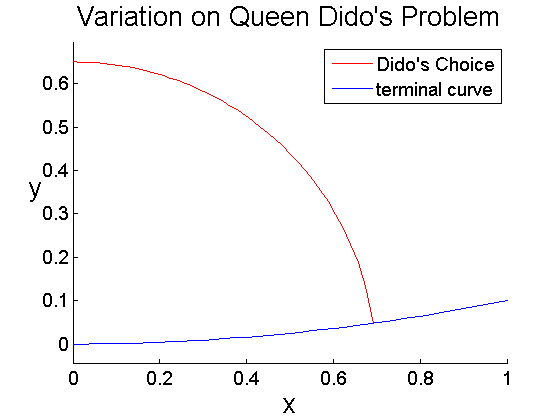
\includegraphics[width=.5\textwidth]{optimalCurve.png}
                        \captionsetup{width=0.8\textwidth}
                        \captionof{figure}{The red curve, of length one, is of the shape to maximize the enclosed region (formed by the red and blue curve).}
                      \end{figure}
\end{enumerate}


\newpage
\subsection*{Matlab Code}{

    \subsection*{queenDidoTerminalCurve.m}{
        \begingroup
        \fontsize{7pt}{7pt}
        \begin{verbatim}
%{
    What we are doing:  Given a Terminal Curve and a bit of 'string' of length L, we wish
    to optimize the region enclosed by out bit of string.  The string can not stretch:
    It's length L and that's that!


    Choose N uniform intervals (hence N+1 points) and discritize the x-axis into uniform
    {x(1),...,x(N+1)}, then we have y(i) as the point on the curve-to-be-optimized at the
    point x(i).

    DecVars: y(1)...y(N+1), x(N+1)  So N+2 Total
    Constraints:
       * y(i)>=0  i = 1,...,N+1
       * 0<=X(N+1)<=L  That is, the last x-point is upper bounded by the curve length
         this is because the maximum length of the curve y(x) forme by the y(i)'s is L,
         hence the final x-point (relating to the final y point) has a maximim length if L

%}
clear all; close all;

%{
    Global variables nessisary to persist variables into the UserFun that Snopt
    uses to converge to the optimal solution.
        N: Number of (uniform) intervals on x-axis.
        f: Function that describes the terminal curve to the modified DIDO problem.
%}
global N f;

%pointer to the snopt userfun; called in the cmex to snopt.
usrfun = 'queenDidoCurveUserFun';


f = @(t) 0.1*t.^2;    %Terminal curve: The last point of the yCurve must lie on this curve
curveLength = 1;      %Exact length of the yCurve
%Arbirtrary upper bound for the area between the decsion curve and the terminal curve
enclosedRegionUpperBound = 300;

%Number of intervals from [x0, xf] where xf is the last node on the x-axis being x(N+1)
N = 40;

%{
    Given a positive integer N, the decesion variables are N+1 points on the curve to be
    made (decesion curve) y(1),...,y(N+1), as well as the last node on the x-axis: x(N+1)
    Hence there are N+2 decesion variables.
%}

%Build an Initial Guess:  For snopt, the initial guess needs to be as a column vector.
%Our initial guess is just a staight line, of length equal to the curveLength, and whose
%last point lies on the terminal curve
xf = curveLength;            %The largest the last value of x can be is the curveLength
yGuess = f(xf)*ones(N+1,1);  %A straight line starting on the y axis ending on the terminal curve
xInit = [ yGuess; xf ];      %initial guess for the Decision Variables


numDecVar = length(xInit);


%{
   Set the lower and upper bounds on the decision variables. SNOPT wants xLow
   and xUpp as column vectors.  Note that the order in which xInit was pack
   determines the ordering of the decision variables.

    All of the decesion variables must lie in the range of 0<=x<=Upp where Upp is some
    arbitrairly large value.  Although, because the length of the decesion curve is always
    fixed (i.e.: it's always 1) the
   upper bound on the final node on the x-axis
%}
xLow = 0*ones(numDecVar,1);
xUpp =  100*ones(numDecVar,1);
xUpp(end) = curveLength;

%{
   Set the lower and upper bounds for the cost function and the constraints
   Note: the order of Flow and Fupp is determined by the packing of the column
   vector F, which is done in the userFun.  F is packed as:
        1) cost function  --inequality constraint: size 1
        2) The length of the decesion curve remains a fixed constant -- size 1
        3) An endpoint constraint: That the last point of the decesion curve must lie
           on the terminal curve
%}
Flow = [ 0;
         curveLength;
         0];    %endponint condition: final y value must lie on the curve f(x)

%upper bounds on the constraints
Fupp = [ enclosedRegionUpperBound;
         curveLength;
         0];    %endpoint condition: final y value must lie on the curve f(x)

%This little 4-line block of setting variables for Snopt are not we do not use;
%we set them to the defaults; ObjRow for example defines which row the
%objective function is located within the constraints col-vec ('F' in the
%userFun)
numConstraints  = length(Flow);
xMul   = zeros(numDecVar,1); xState = zeros(numDecVar,1);
Fmul   = zeros(numConstraints,1); Fstate = zeros(numConstraints,1);
ObjAdd = 0; ObjRow = 1;

%Setting the linear and nonlinear sparsity patterns--this version does not
%supply any of the sparsity patterns; it tells Snopt that every entry of the
%Jacobian needs to be calculated
A  = [];  iAfun = [];  jAvar = [];
[iGfun,jGvar] = find(ones(numConstraints, numDecVar));

%Set the Optimal Parameters for SNOPT. See chapter 7, pg 62 'Optimal Parameters'
%Note we first set 'Defaults' to start SNOPT on a clean-slate; very important!
snset('Defaults');              %You NEED this to flush snopt clean before a run!
snseti('Derivative option', 0); %Telling snopt we know nothing about the jacobian
snseti('Verify level', 3);      %Slows performance but very useful
snset('Maximize');


%Sumary and Solution files; see chapter 8 of SNOPT guide (section 8.8, 8.9)
snprint('result.txt');
snsummary('result.sum');

%Call snopt
solveopt = 1;       %Still have no idea what this flag tells snopt (other than 'optimize')
tic                 %We are going to time snopt
[xOpt,F,xMul,Fmul,INFO] = snoptcmex( solveopt, ...
				                     xInit,xLow,xUpp,xMul,xState, ...
				                     Flow,Fupp,Fmul,Fstate,        ...
				                     ObjAdd,ObjRow,A,iAfun,jAvar,  ...
				                     iGfun,jGvar,usrfun );
runTime=toc;        %we are timing snopt
%%%%%%%%%%%%%%%%%%%%%% Plot Code %%%%%%%%%%%%%%%%%%%%%%

snsummary off; % close the summary .sum file; empties the print buffer
snprint   off; % Closes the print-file .out; empties the print buffer

%Unpack the optimal solution from the column vector Snopt returned
yOpt = xOpt(1:end-1);
xLast = xOpt(end);

%Unpack the initial guess curve, so we can draw it next to the optimal curve
yGuess = xInit(1:end-1);
xGuessDom = linspace(0,curveLength, N+1);   %This is the x-domain used for the guess

%Grab our uniform grid based on the final x-point.  Note that the problem was solved using
%a uniform grid; we just stored the last point durring the computations within the
%userFun.
xGrid = linspace(0, xLast, N+1);

%Plotting the terminal curve along with the optimal curve
hold on;
    plot(xGrid, yOpt, '-r');       %Optimal Curve
    plot(xGuessDom, f(xGuessDom)); %Terminal Curve (last pt on optCurve must lie on this)
%     plot(xGuessDom, yGuess, '-m'); %Initial Guess
    title('Variation on Queen Dido''s Problem', 'FontSize', 20);
    xlabel('x', 'FontSize', 20);
    ylabel('y', 'Rotation', 0, 'FontSize', 20);
    legend('Dido''s Choice', 'terminal curve');
    axis equal;
hold off;

%Just some nicely formated output to the console on the Snopt Run
disp(strcat('Execution time: ', num2str(runTime)));
disp(strcat('SNOPT exited with INFO==', num2str(INFO)));    %see pg 19 snopt manual for INFO

%
% end queenDidoCurve.m
%
        \end{verbatim}
        \endgroup
    }

    \subsection*{queenDidoCurveUserFun.m}{
        \begingroup
        \fontsize{7pt}{7pt}
        \begin{verbatim}
%{
    The UserFun for the Brach Problem. This function is called by SNOPT to
    converge to an optimal solution.  In this function
        1) We pack the nonlinear constraints into F.
        2) We calculate the Jacobian of the constraints with respect to the
           decision variables (variable G).
    In this function, we discritize the dynamics of the Brach problem which were
    set as equality constraints (using Flow and Fupp in the script that calls
    this userFun).


    Inputs:
        decVars: Column vector whose order is determined on how xInit was
                 packed.

    Outputs:
        F: The column vector containing the nonlinear constraints
        G: The Jacobian of the constraints with respect to the decision
           variables; G is a column vector
%}
function [ F, G ] = queenDidoCurveUserFun( decVars )

    global N f;

    %Unpack 'decVars' into meangful variables
    y = decVars(1:end-1);   %The N+1 values that represent points on the decesion curve
    xLast = decVars(end);   %The last value on the x-axis

    %uniform step-size along the x-axis
    deltaX = xLast/N;

    %Calculation of the arcLength of the yCurve:
    %   Sum(i=1 to i=N) of  sqrt( (y(i+1)-y(i))^2 + (x(i+1)-x(i))^2 )
    curveLength = sum(  ( (y(2:end)-y(1:end-1)).^2 + deltaX^2).^(1/2)  );


    %Calculation of the area made by the yCurve (using trapazoidal approximation)
    topCurve = (deltaX/2)*sum( y(2:end)+y(1:end-1) );
    %Calculation of the area made by the terminal curve; note this compuation can not be
    %moved off-line due to the last x-value always changing.  The terminal curve always
    %starts at x=0 since the first y value lies on the y-axis
    bottomCurve = integral(f, 0, xLast);
    areaEnclosed = topCurve - bottomCurve;  %Remember we are maximizing


    %The way F is packed here determines the order of Fupp Flow and the order of
    %the Jacobian of the constraints wrt the decision variables.  F stores the
    %objective function as well as the constraints.
    F = [ areaEnclosed;         %Objective function to maximize is the enclosed area
          curveLength;          %The curve length must be a fixex constant (set in main file)
          y(end) - f(xLast)];   %the last point of the yCurve must lie on the termCurve


     %The Jacobian of the constraints with respect to the decision variables; in
     %this example, we tell Snopt to do it for us.
     G=[];
end
        \end{verbatim}
        \endgroup
    }
}

\end{document} 